\documentclass[conference]{IEEEtran}
\IEEEoverridecommandlockouts

\usepackage{cite}
\usepackage{amsmath,amssymb,amsfonts}
\usepackage{algorithmic}
\usepackage{graphicx}
\usepackage{textcomp}
\usepackage{xcolor}
\usepackage{tikz}
\usetikzlibrary{arrows.meta,positioning,shapes.geometric}

\def\BibTeX{{\rm B\kern-.05em{\sc i\kern-.025em b}\kern-.08em
    T\kern-.1667em\lower.7ex\hbox{E}\kern-.125emX}}

\begin{document}

\title{Anamnesis Humanis untuk Layanan Kesehatan Tropis Indonesia: Benchmark Komparatif DeepSeek dan Gemma dengan Rekomendasi Herbal yang Aman}

\author{\IEEEauthorblockN{1\textsuperscript{st} Sandi Ardiyansah}
\IEEEauthorblockA{\textit{Program Studi Informatika Program Magister} \\
\textit{Universitas Pelita Harapan}\\
Jakarta, Indonesia \\
01679240018@student.uph.edu}
\and
\IEEEauthorblockN{2\textsuperscript{nd} Pujianto Yugopuspito}
\IEEEauthorblockA{\textit{Program Studi Informatika Program Magister} \\
\textit{Universitas Pelita Harapan}\\
Jakarta, Indonesia \\
yugopuspito@uph.edu}}

\maketitle

\begin{abstract}
Masyarakat Indonesia telah menggunakan pengobatan herbal atau jamu selama berabad-abad, sehingga tantangan utama bukan memperkenalkan herbal dari nol, melainkan membantu masyarakat menggunakannya secara lebih aman, terstruktur, dan tidak mudah terpengaruh informasi tidak tervalidasi seperti pesan berantai. Indonesia juga memiliki keanekaragaman hayati yang sangat besar, tetapi pengetahuan herbal tersebut sering belum terhubung dengan asesmen gejala yang sistematis. Paper ini menyajikan chatbot web berbahasa Indonesia yang menerapkan humanizing anamnesis sebelum memberikan rekomendasi herbal, lalu membandingkan dua model bahasa besar lokal, \texttt{deepseek-r1:7b} dan \texttt{gemma4:latest}, di dalam pipeline retrieval-augmented yang dibatasi oleh aturan keselamatan. Purwarupa menggabungkan anamnesis berbasis sesi, logika anti-repetisi, validasi jawaban pasien yang ambigu, batas maksimal tiga pertanyaan lanjutan, knowledge base herbal terkurasi, perankingan model yang deterministik, dan learning log untuk pengembangan LoRA/QLoRA pada tahap berikutnya. Knowledge base yang terindeks berisi 2.781 chunk yang berasal dari 9 record kasus ringan, 10 formula herbal, 13 referensi bahan herbal, 2.731 training record, dan 18 record anamnesis. Korpus SFT/RAG yang tersedia memuat 8.202 contoh gabungan dari data herbal, pengolahan ramuan, penyakit tropis, guidance non-kritis, anamnesis, dan learning log, tetapi paper ini tidak mengevaluasi model yang telah di-fine-tune. Snapshot log runtime yang tersedia pada 29 April 2026 memuat 113 interaksi dual-model (87 follow-up, 25 recommendation, dan 1 sesi red-flag). Gemma lebih sering terpilih secara keseluruhan (42 kemenangan) dibanding DeepSeek (39 kemenangan) dan memiliki tingkat keberhasilan respons yang lebih tinggi (90,0\% versus 75,0\%). DeepSeek tetap kompetitif untuk pembangkitan pertanyaan follow-up, sedangkan Gemma lebih sering menghasilkan rekomendasi akhir yang stabil. Metrik throughput token yang terinstrumentasi masih bersifat preliminary karena hanya tersedia pada subset log awal, sehingga tidak diposisikan sebagai klaim performa statistik final. Sistem ini ditujukan untuk edukasi dan eksplorasi gejala awal, bukan untuk diagnosis definitif, dan secara aktif mengarahkan kasus kritis maupun penyakit dalam ke pemeriksaan tenaga kesehatan.
\end{abstract}

\begin{IEEEkeywords}
anamnesis humanis, layanan kesehatan tropis Indonesia, rekomendasi herbal, retrieval-augmented generation, DeepSeek, Gemma, chatbot medis aman
\end{IEEEkeywords}

\section{Pendahuluan}

\subsection{Latar Belakang dan Motivasi}
Pengobatan tradisional dan herbal tetap relevan di Indonesia karena dekat dengan budaya masyarakat, relatif terjangkau, dan mudah diakses untuk perawatan mandiri di tingkat rumah tangga. Temuan survei nasional menunjukkan bahwa pemanfaatan pengobatan tradisional dan komplementer di Indonesia masih berada pada tingkat yang bermakna \cite{b1}, \cite{b2}. Pada saat yang sama, Organisasi Kesehatan Dunia terus menekankan pentingnya tata kelola pengobatan tradisional yang aman, berpusat pada manusia, dan berbasis bukti \cite{b3}. Namun, pengetahuan perawatan herbal di masyarakat sering terfragmentasi, tidak konsisten terdokumentasi, dan belum terhubung dengan asesmen gejala terstruktur yang mempertimbangkan keselamatan pasien.

Kondisi ini membuka peluang bagi teknologi conversational AI untuk memfasilitasi edukasi herbal yang terstruktur, aman, dan grounded pada pengetahuan yang telah dikurasi. Namun, tantangan utamanya adalah bagaimana merancang chatbot yang bertanggung jawab secara klinis — yang tidak langsung merekomendasikan herbal, tetapi terlebih dahulu melakukan anamnesis yang ringkas, aman, tidak repetitif, dan grounded pada knowledge base yang tersedia.

\subsection{Rumusan Masalah dan Pertanyaan Penelitian}
\textbf{Rumusan Masalah:} Dalam konteks layanan kesehatan tropis Indonesia, keluhan publik seperti demam, batuk, sakit tenggorokan, diare, ruam gatal, dan pegal badan dapat merepresentasikan kondisi ringan, tetapi juga dapat tumpang tindih dengan kondisi serius seperti dengue, dehidrasi, infeksi akut, atau tanda bahaya lain yang membutuhkan pemeriksaan formal. Chatbot yang langsung merekomendasikan herbal tanpa terlebih dahulu menggali durasi, tingkat keparahan, gejala penyerta, dan tanda bahaya tidak bertanggung jawab secara klinis. Sebaliknya, chatbot yang melakukan anamnesis berlebihan menjadi tidak praktis dan tidak efisien dalam deployment lokal. Oleh karena itu, diperlukan sistem yang dapat menyeimbangkan tiga kebutuhan yang saling bertentangan: (1) anamnesis yang humanis dan tidak repetitif, (2) keselamatan klinis yang ketat dengan grounding pada knowledge base herbal, dan (3) praktikalitas dalam deployment lokal dengan latensi yang wajar.

\textbf{Pertanyaan Penelitian Utama:} Bagaimana merancang chatbot edukasi herbal berbahasa Indonesia yang tidak langsung memberi rekomendasi, tetapi terlebih dahulu melakukan anamnesis ringkas, aman, tidak repetitif, grounded pada knowledge base herbal yang terkurasi, dan tetap praktis dijalankan secara lokal?

Pertanyaan ini dapat diurai menjadi sub-pertanyaan berikut:
\begin{enumerate}
\item Bagaimana merancang alur anamnesis yang terasa humanis, menghindari repetisi pertanyaan, dan mengekstrak informasi gejala kritis (durasi, keparahan, tanda bahaya) dalam jumlah pertanyaan yang minimal?
\item Bagaimana mengintegrasikan retrieval-augmented generation (RAG) dan multi-model assessment untuk memastikan bahwa rekomendasi herbal selalu grounded pada knowledge base dan dibatasi oleh kriteria keselamatan yang ketat?
\item Bagaimana mengoperasionalkan dua model bahasa besar lokal secara bersamaan untuk meningkatkan robustness respons dan mengurangi hallucination, sambil tetap mempertahankan latensi yang praktis untuk deployment lokal?
\item Bagaimana mengukur efektivitas sistem melalui benchmark operasional (bukan hanya benchmark offline) dan mengumpulkan learning log untuk pengembangan incremental selanjutnya?
\end{enumerate}

\subsection{Tujuan Penelitian}
Tujuan penelitian ini adalah merancang dan mengevaluasi sebuah purwarupa chatbot edukasi herbal berbahasa Indonesia yang menerapkan anamnesis-first interaction, safety-constrained retrieval-augmented generation (RAG), dan dual-model runtime comparison menggunakan dua model open-source lokal (\texttt{deepseek-r1:7b} dan \texttt{gemma4:latest}). Sistem dirancang untuk (1) melakukan anamnesis ringkas dan humanis sebelum memberikan rekomendasi herbal, (2) menghindari rekomendasi yang tidak grounded pada knowledge base terkurasi, (3) memberikan respons yang aman dan non-repetitif, dan (4) tetap praktis dijalankan pada mesin lokal dengan latensi yang wajar. Evaluasi berfokus pada perbandingan operasional antara kedua model melalui runtime log nyata, bukan benchmark offline, serta pengumpulan learning log untuk pengembangan incremental selanjutnya.

\subsection{Tantangan dan Keterbatasan Pendekatan Existing}
Chatbot medis history-taking berbasis LLM telah menunjukkan hasil yang menjanjikan \cite{b4}. Namun, tiga tantangan utama muncul ketika membangun sistem untuk konteks herbal lokal Indonesia:

Sistem medis berbasis LLM mutakhir umumnya mengambil salah satu dari dua arah. ChatDoctor, misalnya, menekankan fine-tuning model percakapan medis berbasis dialog pasien-dokter dan retrieval pengetahuan medis \cite{b20}. MEDRAG/MIRAGE menempatkan retrieval sebagai fokus utama untuk medical QA berskala besar \cite{b21}. AMIE dari Google menargetkan diagnostic dialogue yang lebih komprehensif dengan evaluasi dokter spesialis dan pasien standar \cite{b22}. Berbeda dari pendekatan tersebut, purwarupa ini tidak berusaha menjadi model diagnosis umum; kontribusinya adalah memisahkan tahap anamnesis, safety gate, retrieval herbal lokal, dan ranking multi-model untuk konteks edukasi awal keluhan ringan di Indonesia.

\textbf{Tantangan 1: Humanisasi Anamnesis Tanpa Repetisi.} Chatbot yang bergantung pada satu model tunggal menghasilkan respons yang mudah menjadi repetitif atau generik, sehingga mengurangi nuansa ``seperti dokter'' pada anamnesis. Model single tidak memiliki mekanisme untuk menyimpan dan menghindari pertanyaan yang sudah diajukan dalam turn sebelumnya.

\textbf{Tantangan 2: Grounding pada Knowledge Base Lokal.} Keluaran model dapat melenceng dari pengetahuan herbal yang valid dan terdokumentasi bila tidak dibatasi oleh retrieval terhadap knowledge base. Hallucination adalah risiko tinggi pada domain kesehatan \cite{b6}. Retrieval-augmented generation (RAG) menjadi lapisan yang relevan \cite{b5}, tetapi implementasinya harus ringan dan sesuai dengan kerangka deployment lokal.

\textbf{Tantangan 3: Tradeoff Kualitas dan Latensi pada Deployment Lokal.} Menjalankan model besar secara lokal (tanpa API cloud) menimbulkan tradeoff antara kualitas inferensi dan latensi response. Benchmark offline berbasis prompt statis tidak mencerminkan perilaku sistem di production. Diperlukan benchmark operasional yang tertanam langsung dalam purwarupa yang berjalan.

\subsection{Kontribusi Penelitian}
Paper ini menjawab pertanyaan penelitian di atas dengan mengusulkan dan mengevaluasi sebuah purwarupa chatbot anamnesis-first yang terintegrasi dengan benchmark komparatif multi-model. Sistem membandingkan dua model lokal yang dijalankan melalui Ollama, yaitu \texttt{deepseek-r1:7b} dan \texttt{gemma4:latest}, setelah keduanya menerima ringkasan anamnesis terstruktur dan konteks herbal retrieval yang sama. Keluaran masing-masing model diberi skor secara deterministik berdasarkan safety, grounding, completeness, relevance, language quality, dan kriteria khusus tugas. Hanya kandidat dengan skor tertinggi yang ditampilkan kepada pengguna. Seluruh interaksi tercatat dalam learning log untuk pengembangan LoRA/QLoRA pada tahap berikutnya.

Kontribusi utama paper ini adalah sebagai berikut:
\begin{enumerate}
\item Mengusulkan arsitektur chatbot anamnesis-first berbahasa Indonesia yang menjawab pertanyaan penelitian utama, dengan mekanisme anti-repetisi, batas pertanyaan yang jelas (maksimal tiga follow-up), dan safety gate yang ketat sebelum rekomendasi herbal.
\item Mengintegrasikan humanizing anamnesis dengan RAG, perankingan multi-model yang deterministik, dan batas keselamatan untuk use-case non-kritis, serta mendokumentasikan trade-off design.
\item Melaporkan perbandingan operasional antara DeepSeek-R1 7B dan Gemma4 menggunakan runtime log nyata dari purwarupa yang berjalan (bukan impresi subjektif berbasis prompt), mencakup perilaku per-tahap percakapan, error rate, skor grounding, dan latensi inferensi.
\item Menginstrumentasi purwarupa dengan structured learning log, capture umpan balik pengguna, dan aset pelatihan terformat (SFT/LoRA) untuk pengembangan incremental, menciptakan jembatan langsung antara benchmarking operasional dan fine-tuning model selanjutnya.
\end{enumerate}


Walaupun implementasi dapat memanggil \texttt{gpt-4o} secara opsional, paper ini memfokuskan pembahasan pada pasangan model lokal default karena tujuan risetnya adalah benchmark antara model yang realistis untuk deployment lokal pada layanan kesehatan Indonesia.

\section{Desain Sistem dan Aset Data}
\subsection{Ruang Lingkup dan Prinsip Perancangan}
Purwarupa ini adalah chatbot web berbahasa Indonesia untuk eksplorasi gejala awal dan edukasi herbal yang aman. Sistem tidak ditujukan untuk menegakkan diagnosis penyakit, meresepkan obat, atau menangani kondisi gawat darurat. Ruang lingkup yang didukung meliputi keluhan tropis ringan dan keluhan rawat jalan non-kritis yang berdekatan, sedangkan kondisi kritis, penyakit dalam, dan progresivitas berat diarahkan ke respons rujukan medis atau red-flag. Dengan demikian, keluaran herbal selalu bersifat kondisional: sistem harus terlebih dahulu memastikan bahwa kasus cukup ringan, non-kritis, dan grounded pada knowledge base terkurasi.

Tiga prinsip perancangan mendasari implementasi ini. Pertama, anamnesis harus terasa humanis, bukan robotik; karena itu sistem menyimpan answered slots dan menghindari pertanyaan yang sama berulang kali. Kedua, setiap respons herbal harus dapat diaudit; karena itu generator dibatasi oleh konteks retrieval. Ketiga, sistem harus tetap praktis pada mesin lokal; karena itu benchmark difokuskan pada dua model lokal dan retrieval dibuat dengan komponen yang ringan.

\subsection{Aset Knowledge Base}
Knowledge base menggabungkan aset referensi, anamnesis, dan training yang disimpan di folder data proyek. Tabel \ref{tab:data_assets_id} merangkum aset yang saat ini telah terindeks dan siap digunakan untuk training.

\begin{table}[t]
\caption{Aset Knowledge dan Training Saat Ini}
\label{tab:data_assets_id}
\centering
\footnotesize
\setlength{\tabcolsep}{3pt}
\begin{tabular}{|p{2.05cm}|c|p{3.15cm}|}
\hline
\textbf{Aset} & \textbf{Jumlah} & \textbf{Peran dalam Sistem} \\
\hline
Record kasus ringan & 9 & Pengait utama antara gejala dan kandidat herbal \\
\hline
Record formula herbal & 10 & Nama formula, komposisi, dan catatan keamanan \\
\hline
Record referensi bahan & 13 & Konteks grounding di level bahan herbal \\
\hline
Training record & 2.731 & Guidance herbal, detail pengolahan, dan guidance penyakit tropis serta non-kritis \\
\hline
Record anamnesis & 18 & Panduan pertanyaan follow-up dan red-flag \\
\hline
Knowledge chunk terindeks & 2.781 & Total chunk yang disimpan di ChromaDB \\
\hline
Korpus SFT/RAG gabungan & 8.202 & Contoh training gabungan untuk LoRA/QLoRA dan evaluasi RAG \\
\hline
\end{tabular}
\end{table}

Basis referensi dimulai dari case herbal ringan, lalu diperluas dengan detail pengolahan, materi kesehatan tropis, dan kondisi non-kritis yang lebih luas. Sumber yang digunakan mencakup artikel edukasi dan layanan kesehatan Kemenkes/Keslan dan AyoSehat \cite{b14}, JDIH Kemenkes untuk konteks Formularium Obat Herbal Asli Indonesia \cite{b15}, ringkasan keamanan NCCIH \cite{b16}, literatur PubMed, serta guidance penyakit dari MedlinePlus \cite{b17}, WHO \cite{b18}, CDC \cite{b19}, dan dokumen penyakit tropis lokal yang diparsing ke format terstruktur. Data anamnesis dibangun dari sumber resmi tersebut dan beberapa rujukan pendukung untuk pertanyaan gejala, tanda bahaya, dan tindakan triase. Setiap record menyimpan metadata sumber, level evidensi, dan catatan kewaspadaan agar retrieval dapat diaudit kembali.

Data ini diperlakukan sebagai knowledge base terkurasi teknis, bukan sebagai clinical guideline final. Pada versi ini belum dilakukan validasi formal oleh panel dokter, dokter herbal, atau farmakolog klinis. Karena itu, klaim sistem dibatasi pada edukasi, triase awal, dan rekomendasi pendamping untuk keluhan ringan; validasi pakar dan audit klinis prospektif ditempatkan sebagai kebutuhan sebelum deployment produksi.

Hal ini penting karena objective sistem saat ini tidak lagi dibatasi hanya pada label penyakit tropis, melainkan mendukung keluhan ringan di luar penyakit tropis, sambil tetap mengecualikan penyakit dalam dan kondisi kritis.

\subsection{Arsitektur Runtime}
Pipeline runtime terdiri dari session synchronization, analisis anamnesis, scope control, retrieval, komparasi model, composition rekomendasi, dan learning capture. Alur sederhananya ditunjukkan pada Gambar \ref{fig:workflow_id}. Alih-alih memakai generator medis monolitik lama, arsitektur saat ini melakukan multi-model assessment hanya setelah input diringkas menjadi konteks anamnesis terstruktur.

\begin{figure}[t]
\centering
\resizebox{\columnwidth}{!}{%
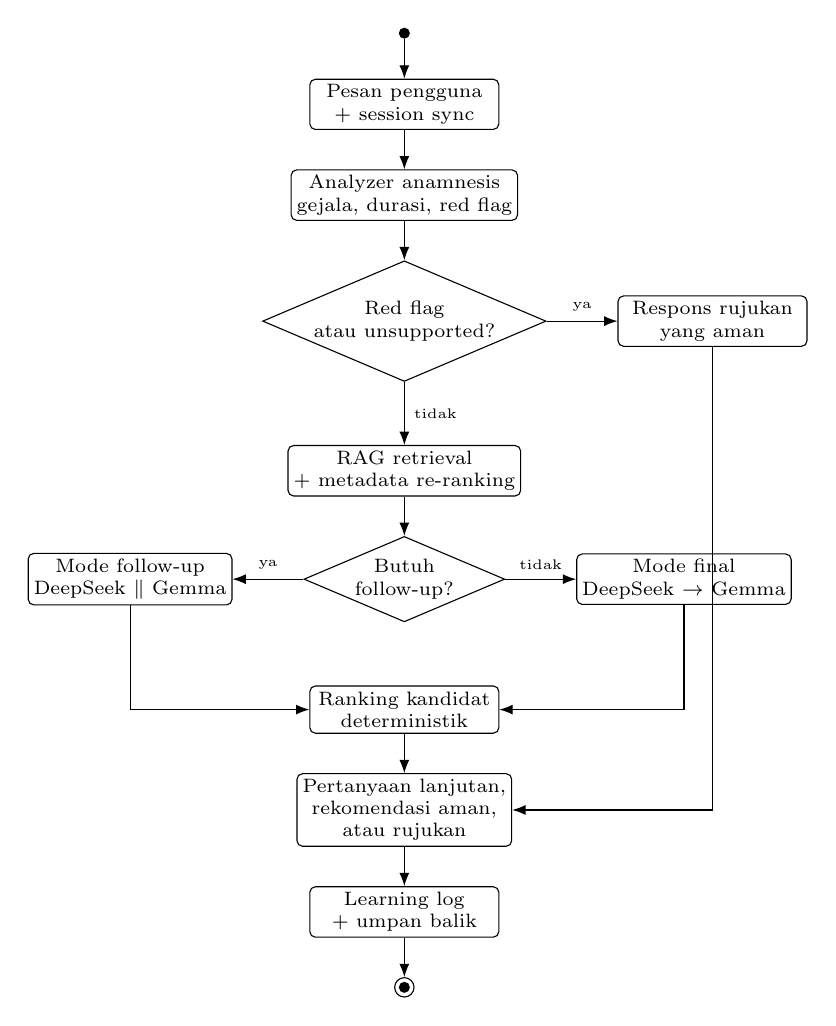
\begin{tikzpicture}[
node distance=5mm and 9mm,
umlstart/.style={circle, fill=black, minimum size=4pt, inner sep=0pt},
umlend/.style={circle, draw=black, minimum size=7pt, inner sep=0pt,
path picture={\fill (path picture bounding box.center) circle (2pt);}},
umlact/.style={draw, rounded corners=2pt, align=center, minimum width=24mm,
minimum height=6mm, font=\scriptsize, inner sep=2pt},
umldec/.style={draw, diamond, aspect=2.35, align=center, font=\scriptsize,
inner sep=0.5pt},
umlarrow/.style={-Latex, line width=0.4pt}
]
\node[umlstart] (start) {};
\node[umlact, below=of start] (sync) {Pesan pengguna\\+ session sync};
\node[umlact, below=of sync] (anam) {Analyzer anamnesis\\gejala, durasi, red flag};
\node[umldec, below=of anam] (safety) {Red flag\\atau unsupported?};
\node[umlact, right=of safety] (referral) {Respons rujukan\\yang aman};
\node[umlact, below=8mm of safety] (retrieval) {RAG retrieval\\+ metadata re-ranking};
\node[umldec, below=of retrieval] (need) {Butuh\\follow-up?};
\node[umlact, left=of need] (follow) {Mode follow-up\\DeepSeek $\parallel$ Gemma};
\node[umlact, right=of need] (final) {Mode final\\DeepSeek $\rightarrow$ Gemma};
\node[umlact, below=8mm of need] (rank) {Ranking kandidat\\deterministik};
\node[umlact, below=of rank] (answer) {Pertanyaan lanjutan,\\rekomendasi aman,\\atau rujukan};
\node[umlact, below=of answer] (log) {Learning log\\+ umpan balik};
\node[umlend, below=of log] (end) {};

\draw[umlarrow] (start) -- (sync);
\draw[umlarrow] (sync) -- (anam);
\draw[umlarrow] (anam) -- (safety);
\draw[umlarrow] (safety) -- node[above, font=\tiny] {ya} (referral);
\draw[umlarrow] (referral) |- (answer);
\draw[umlarrow] (safety) -- node[right, font=\tiny] {tidak} (retrieval);
\draw[umlarrow] (retrieval) -- (need);
\draw[umlarrow] (need) -- node[above, font=\tiny] {ya} (follow);
\draw[umlarrow] (need) -- node[above, font=\tiny] {tidak} (final);
\draw[umlarrow] (follow) |- (rank);
\draw[umlarrow] (final) |- (rank);
\draw[umlarrow] (rank) -- (answer);
\draw[umlarrow] (answer) -- (log);
\draw[umlarrow] (log) -- (end);
\end{tikzpicture}%
}
\caption{Diagram aktivitas UML alur runtime chatbot yang diusulkan.}
\label{fig:workflow_id}
\end{figure}

Lapisan session synchronization merupakan tambahan praktis yang muncul dari proses pengembangan. Frontend mengirimkan kembali state percakapan ke backend pada setiap request agar sistem tetap bisa mempertahankan histori follow-up walaupun halaman di-refresh atau service di-restart. Mekanisme ini juga membuat comparator dapat memberi penalti terhadap pertanyaan duplikat secara lebih andal.

\section{Anamnesis Humanis dan Metode Benchmark}
\subsection{Pengendali Anamnesis}
Pengendali anamnesis mengekstrak gejala yang hadir, gejala yang disangkal, ekspresi durasi, dan tanda bahaya dari setiap turn pengguna. Sistem juga menyimpan answered slots seperti ``demam sudah disebut,'' ``durasi sudah disebut,'' dan ``tanda bahaya sudah disangkal.'' Slot-slot ini dimasukkan ke prompt model agar sistem dapat menanyakan follow-up yang lebih spesifik, bukan mengulang pertanyaan generik seperti menanyakan demam ketika pengguna telah menyebut demam di awal.

Kebijakan percakapan memiliki tiga state. Pada state pertama, red-flag detection mem-bypass komparasi model dan langsung menghasilkan respons rujukan yang aman. Pada state kedua, jika informasi masih belum lengkap dan anggaran pertanyaan belum mencapai tiga, comparator meminta satu pertanyaan follow-up dari masing-masing model. Pada state ketiga, ketika informasi sudah cukup atau batas tiga pertanyaan telah tercapai, sistem memaksa jalur final recommendation ranking. Desain ini mencegah percakapan berputar tanpa akhir, tetapi tetap menjaga ketajaman anamnesis. Implementasi terbaru juga menambahkan guardrail percakapan untuk menjelaskan ulang pertanyaan ketika pengguna menyatakan bingung, meminta klarifikasi ketika angka suhu tidak realistis, dan menafsirkan jawaban pendek seperti ``tidak ada'' berdasarkan pertanyaan anamnesis sebelumnya.

\subsection{Retrieval dan Perankingan Model}
RAG diimplementasikan dengan embedding lokal yang ringan dan ChromaDB. Motivasi utama pemilihan ini adalah kepraktisan operasional, bukan semata-mata memaksimalkan kualitas retrieval semantik dengan layanan embedding besar. Sentence encoder ringan dan model distilasi tetap relevan sebagai titik acuan tradeoff tersebut \cite{b7}, \cite{b8}. Item yang diretrieval mencakup case record, formula, referensi bahan, training record, dan record anamnesis, yang kemudian diurutkan ulang memakai sinyal metadata seperti overlap gejala, case hint, level evidensi, dan kecocokan formula.

Kedua model kandidat menerima prompt medis yang sama: turn percakapan terbaru, ringkasan anamnesis, heuristik red-flag, daftar follow-up yang sudah pernah ditanyakan, dan konteks retrieval. Masing-masing model wajib mengembalikan assessment JSON terstruktur, bukan prosa bebas. Lapisan ranking lalu menghitung skor khusus tugas. Untuk turn follow-up, skor agregat dirumuskan sebagai
\begin{align}
S_f &= 0.25s + 0.20g + 0.16c + 0.16r \nonumber \\
&\quad + 0.08l + 0.05q + 0.10n,
\end{align}
dengan $s$ menyatakan safety, $g$ grounding, $c$ completeness, $r$ relevance, $l$ language quality, $q$ question quality, dan $n$ non-repetition.

Untuk turn final recommendation, skornya menjadi
\begin{align}
S_r &= 0.28s + 0.22g + 0.20c + 0.14r \nonumber \\
&\quad + 0.08l + 0.08h,
\end{align}
dengan $h$ menyatakan herbal fit. Desain ini sengaja memberi bobot terbesar pada safety dan grounding, sesuai dengan profil risiko tugas kesehatan ini.

Bobot pada kedua persamaan ditetapkan sebagai heuristik a-priori berbasis prioritas risiko, bukan hasil optimasi statistik terhadap log benchmark. Safety dan grounding diberi bobot terbesar karena kegagalan pada dua aspek ini memiliki konsekuensi paling serius pada domain kesehatan; completeness dan relevance ditempatkan sebagai lapisan kualitas utama berikutnya, sedangkan language quality, question quality, non-repetition, dan herbal fit berfungsi sebagai tie-breaker operasional. Bobot tersebut tidak dituning untuk memaksimalkan kemenangan model tertentu, sehingga ranking dapat dipahami sebagai kebijakan desain yang konservatif dan dapat diaudit, bukan estimator performa klinis final.

Nilai komponen skor tidak berasal dari self-evaluation model dan tidak menggunakan LLM-as-a-judge. Semua komponen dihitung oleh script deterministik setelah output JSON model diparsing. Komponen safety memberi kredit pada scope \emph{critical}/\emph{internal medicine}, flag rujukan medis, keberadaan red flag, dan bahasa keselamatan seperti arahan ke tenaga kesehatan atau disclaimer. Komponen grounding dihitung dari overlap token antara dugaan kondisi, nama ramuan, bahan, \emph{source hint}, dan judul konteks retrieval teratas. Completeness mengecek kelengkapan field wajib sesuai mode, misalnya follow-up question dan rationale pada mode anamnesis, atau final answer, warning, herbal, preparation, dan dosage pada mode rekomendasi. Relevance mengukur overlap token antara pesan pengguna, gejala yang terdeteksi, kandidat pertanyaan/jawaban, dan konteks retrieval. Language quality pada versi ini adalah heuristik panjang respons yang menolak output terlalu pendek atau terlalu panjang. Question quality mengecek apakah pertanyaan tunggal, berbentuk tanya, dan masih berada dalam anggaran follow-up, sedangkan non-repetition memberi penalti pada pertanyaan yang mengulang gejala, durasi, atau pertanyaan sebelumnya. Herbal fit memberi kredit ketika nama ramuan dan bahan yang diusulkan muncul pada konteks retrieval dan disertai cara pengolahan serta dosis. Dengan demikian, ranking bersifat rule-based, auditable, dan dapat direproduksi dari learning log.

\subsection{Safety, Umpan Balik, dan Loop Training}
Sistem memblokir rekomendasi ketika scope termasuk \emph{critical}, \emph{internal medicine}, atau \emph{unsupported}. Bahkan saat scope masih \emph{supported}, jawaban akhir tetap harus memuat bahasa keselamatan yang konservatif dan tetap terikat pada konteks herbal yang diretrieval. Hal ini selaras dengan kekhawatiran RAG di domain kesehatan \cite{b6}, sekaligus sejalan dengan gagasan evaluasi RAG seperti grounding dan faithfulness \cite{b9}.

Tiga kelas log menjadi inti benchmark ini. Pertama, \texttt{conversation\_turns.jsonl} menyimpan turn pengguna dan assistant. Kedua, \texttt{dual\_llm\_interactions.jsonl} menyimpan keluaran kandidat, skor, model terpilih, dan latensi. Ketiga, \texttt{kb\_enrichment\_candidates.jsonl} menyimpan usulan pengetahuan baru yang masih membutuhkan kurasi manusia. File terpisah \texttt{recommendation\_feedback.jsonl} menyimpan apakah pengguna merasa terbantu oleh rekomendasi yang diberikan. Seluruh log ini membangun jembatan langsung antara benchmarking runtime dan pengembangan LoRA/QLoRA pada tahap selanjutnya \cite{b10}, \cite{b11}.

\section{Pengaturan Eksperimen dan Hasil}
\subsection{Snapshot Benchmark}
Benchmark pada paper ini menggunakan snapshot log operasional yang tersedia pada 29 April 2026. Pasangan lokal default adalah \texttt{deepseek-r1:7b} dan \texttt{gemma4:latest}. Komparasi berbasis GPT memang ada di codebase, tetapi tidak dimasukkan ke benchmark utama karena sifatnya opsional dan bukan target deployment lokal default. Snapshot yang dianalisis berisi 113 interaksi dual-model yang tercatat, terdiri dari 87 respons follow-up, 25 final recommendation, dan 1 respons red-flag.

Benchmark ini bukan benchmark laboratorium dengan replay prompt yang seragam, melainkan benchmark operasional dari purwarupa yang benar-benar berjalan. Konsekuensinya, data menjadi lebih ``kotor'' tetapi juga lebih realistis, karena mencakup run yang sukses, pemakaian fallback, timeout, dan perilaku pemulihan state. Tabel \ref{tab:primary_models_id} melaporkan perbandingan model utamanya.

\begin{table}[t]
\caption{Benchmark Model Utama dari Runtime Log}
\label{tab:primary_models_id}
\centering
\scriptsize
\setlength{\tabcolsep}{2pt}
\begin{tabular}{|p{1.6cm}|c|c|c|c|c|}
\hline
\textbf{Model} & \textbf{N} & \textbf{Win} & \textbf{OK} & \textbf{Skor} & \textbf{Lat.} \\
\hline
DeepSeek-R1 7B & 88 & 39 & 75.0\% & 0.5756 & 23.76 s \\
\hline
Gemma4 latest & 90 & 42 & 90.0\% & 0.5764 & 24.66 s \\
\hline
\end{tabular}
\end{table}

Gemma menunjukkan rerata skor yang sedikit lebih baik dan robustness yang lebih tinggi, dengan error rate yang lebih rendah pada environment yang sama. Pada snapshot terbaru, rerata latensi respons sukses DeepSeek sedikit lebih rendah daripada Gemma, tetapi selisihnya masih berada pada orde puluhan detik karena keduanya berjalan lokal melalui Ollama dan dipengaruhi panjang prompt serta fallback.

\subsection{Perilaku Berdasarkan Tahap Percakapan}
Jumlah kemenangan total menyembunyikan perbedaan penting antar tahap. DeepSeek dan Gemma tidak mendominasi bagian workflow yang sama. Tabel \ref{tab:stage_wins_id} menunjukkan distribusi model terpilih berdasarkan tahap respons.

\begin{table}[t]
\caption{Model Terpilih Berdasarkan Tahap Runtime}
\label{tab:stage_wins_id}
\centering
\footnotesize
\begin{tabular}{|l|c|c|}
\hline
\textbf{Output Terpilih} & \textbf{Follow-up} & \textbf{Recommendation} \\
\hline
DeepSeek-R1 7B & 39 & 0 \\
\hline
Gemma4 latest & 31 & 11 \\
\hline
Model fallback & 5 & 11 \\
\hline
Tidak ada pemenang & 12 & 3 \\
\hline
\end{tabular}
\end{table}

Pemisahan per tahap ini memberi interpretasi perilaku yang menarik. DeepSeek-R1 7B lebih kompetitif pada generasi follow-up, yaitu ketika ketajaman pertanyaan dan eksplorasi gejala lebih dominan. Sebaliknya, Gemma4 latest lebih stabil pada penyusunan final recommendation, yaitu saat keluaran harus ringkas, aman, grounded, dan lengkap. Temuan ini konsisten dengan tujuan sistem dual-model: pembentukan pertanyaan lanjutan dan penyusunan jawaban akhir belum tentu diuntungkan oleh perilaku model yang sama.

\subsection{Metrik Inferensi}
Frontend kini menampilkan metadata komparasi model seperti provider, total latency, dan metrik inferensi detail ketika tersedia. Untuk model yang berjalan di atas Ollama, sistem mencatat \texttt{total\_duration}, \texttt{load\_duration}, \texttt{prompt\_eval\_count}, \texttt{prompt\_eval\_duration}, \texttt{eval\_count}, dan \texttt{eval\_duration}, lalu menurunkan nilai token-per-second. Karena instrumentasi ini baru diaktifkan setelah sebagian log lama sudah terbentuk, baru subset awal saja yang memiliki metrik detail tersebut. Tabel \ref{tab:inference_metrics_id} melaporkan rerata awalnya.

\begin{table}[t]
\caption{Metrik Inferensi Awal yang Sudah Diinstrumentasi}
\label{tab:inference_metrics_id}
\centering
\footnotesize
\begin{tabular}{|l|c|c|}
\hline
\textbf{Metrik} & \textbf{DeepSeek-R1 7B} & \textbf{Gemma4 latest} \\
\hline
Prompt eval rate & 197.89 tok/s & 292.83 tok/s \\
\hline
Generation eval rate & 20.27 tok/s & 26.78 tok/s \\
\hline
Sampel terinstrumentasi & 10 & 11 \\
\hline
\end{tabular}
\end{table}

Angka awal ini belum cukup besar untuk menjadi klaim throughput yang definitif. Metrik token-per-second pada Tabel \ref{tab:inference_metrics_id} hanya diperlakukan sebagai bukti bahwa instrumentasi inferensi sudah berjalan, bukan sebagai uji statistik performa model. Evaluasi throughput yang lebih kuat perlu menjalankan replay offline atau load test terkontrol terhadap 50--100 prompt historis dengan seed, model, dan mesin yang sama. Yang lebih penting pada versi ini, instrumentasi tersebut membuat benchmark ke depan dapat diaudit secara lebih baik, karena paper tidak lagi hanya bergantung pada kesan subjektif ``terasa lebih cepat''.

\subsection{Outcome Humanizing dan Safety}
Benchmark ini tidak hanya membahas model mana yang lebih cepat. Perbaikan pada level sistem juga penting. Implementasi saat ini memiliki tiga pengaman praktis yang secara langsung meningkatkan kualitas percakapan selama pengembangan:
\begin{itemize}
\item \textbf{anti-repetition:} kandidat follow-up diberi penalti bila menanyakan gejala atau durasi yang sudah disebut pengguna;
\item \textbf{session synchronization:} state frontend dikirim ulang ke backend agar histori follow-up tidak hilang setelah restart;
\item \textbf{clarification guardrail:} pesan seperti ``tidak mengerti'' tidak diproses sebagai gejala baru, tetapi dijawab dengan penjelasan ulang pertanyaan anamnesis dalam bahasa awam;
\item \textbf{input sanity check:} angka suhu yang tidak mungkin secara fisiologis, misalnya 89 derajat, diperlakukan sebagai salah ketik dan diminta klarifikasi;
\item \textbf{contextual short answer:} jawaban singkat seperti ``tidak ada'' ditafsirkan terhadap pertanyaan terakhir, sehingga sistem dapat menyimpan bahwa tanda bahaya tertentu sudah disangkal;
\item \textbf{forced completion:} sistem berpindah ke final recommendation ketika tiga turn follow-up telah tercapai atau coverage informasi sudah cukup.
\end{itemize}

Kontrol tersebut penting bagi ``anamnesis humanis,'' karena pertanyaan yang repetitif atau pelupa cepat merusak ilusi percakapan yang terasa seperti dokter. Modul feedback juga sudah menangkap record rekomendasi pertama yang dinilai membantu, walaupun jumlah sampel ini masih terlalu kecil untuk dijadikan studi pengguna formal.

\section{Pembahasan}
Benchmark menunjukkan bahwa desain dual-model tetap berguna walaupun kedua model memiliki rerata skor yang berdekatan. Gemma4 latest dan DeepSeek-R1 7B nyaris seimbang pada skor agregat, tetapi perilaku operasionalnya berbeda. Gemma lebih robust dan lebih sering terpilih secara keseluruhan, sedangkan DeepSeek lebih kuat untuk eksplorasi follow-up. Hal ini menyiratkan bahwa chatbot kesehatan masa depan tidak seharusnya mengasumsikan satu model selalu unggul pada semua tahap interaksi.

Hasil saat ini juga mendukung keputusan untuk menjalankan follow-up secara paralel dan final recommendation secara berurutan. Jika kedua tahap dijalankan dalam mode yang sama, sistem berisiko mengalami latensi yang lebih tinggi atau stabilitas yang lebih rendah pada mesin lokal. Karena itu, strategi eksekusi hibrid ini bukan sekadar kompromi engineering, melainkan keputusan desain yang dipandu oleh perilaku deployment nyata.

Terdapat beberapa keterbatasan. Pertama, benchmark ini didasarkan pada runtime log operasional, bukan pada gold-standard evaluation set yang seimbang. Kedua, instrumentasi throughput baru mencakup subset awal setelah logging metrik ditambahkan, sehingga hasil token-per-second harus dibaca sebagai preliminary. Ketiga, dataset feedback masih kecil dan belum mendukung klaim kuat mengenai perceived usefulness. Keempat, lapisan retrieval masih mengutamakan deployment lokal yang praktis, sehingga embedding medis multilingual yang lebih baik masih berpotensi meningkatkan versi berikutnya.

Keterbatasan paling penting untuk domain medis adalah belum adanya baseline evaluasi pakar. Walaupun sistem mencatat user feedback dan melakukan scoring deterministik, hal tersebut belum setara dengan penilaian klinis. Evaluasi berikutnya perlu melibatkan dokter umum, dokter penyakit tropis, atau tenaga kesehatan tradisional/herbalis terlatih untuk memberi rating terhadap keamanan triase, kecukupan anamnesis, grounding rekomendasi, dan potensi misleading advice. Desain evaluasi yang lebih kuat dapat memakai vignette klinis berlabel, inter-rater agreement, serta analisis kesalahan terhadap kasus demam, diare, ruam, batuk, dan gejala tropis yang berisiko tinggi.

Walaupun demikian, purwarupa saat ini sudah menunjukkan pola deployment LLM yang layak publikasi untuk aplikasi bantuan kesehatan Indonesia: anamnesis terlebih dahulu, retrieval sebelum rekomendasi, penolakan eksplisit terhadap red flag, perankingan deterministik lintas model, dan log yang dapat digunakan kembali untuk adaptasi LoRA/QLoRA.

\section{Kesimpulan}
Paper ini menyajikan chatbot kesehatan berbahasa Indonesia yang berorientasi pada anamnesis terlebih dahulu untuk keluhan tropis ringan dan keluhan non-kritis, dengan rekomendasi herbal aman sebagai titik akhir edukatif, bukan tindakan diagnostik. Benchmark membandingkan \texttt{deepseek-r1:7b} dan \texttt{gemma4:latest} di dalam pipeline RAG yang sama. Pada snapshot runtime yang memuat 113 interaksi dan tersedia pada 29 April 2026, Gemma lebih sering terpilih secara keseluruhan dan memiliki successful-response rate yang lebih baik. DeepSeek tetap kompetitif, terutama untuk pembangkitan pertanyaan follow-up, sehingga kekuatan model terbukti bergantung pada tahap dialognya.

Kontribusi yang lebih luas dari paper ini bersifat metodologis. Dengan menggabungkan humanizing anamnesis, kontrol anti-repetisi, grounding berbasis RAG, scoring yang deterministik, dan learning log, sistem membangun loop benchmark yang praktis antara deployment dan refinement model di masa depan. Evaluasi pada paper ini tetap dibatasi pada arsitektur RAG dan benchmark operasional model lokal, bukan pada klaim keberhasilan fine-tuning. Hal ini menjadikan purwarupa sebagai landasan yang kuat untuk evaluasi yang lebih besar dengan pakar, embedding medis yang lebih kuat, dan adaptasi domain berbasis LoRA untuk chatbot kesehatan Indonesia.

\section*{Ucapan Terima Kasih}
Penulis mengucapkan terima kasih kepada Program Studi Informatika Program Magister Universitas Pelita Harapan atas dukungan terhadap riset ini pada pengembangan sistem chatbot kesehatan yang aman dan dapat diaudit.

\begin{thebibliography}{00}
\bibitem{b1} S. Pengpid and K. Peltzer, ``Utilization of traditional and complementary medicine in Indonesia: Results of a national survey in 2014--15,'' \emph{Complementary Therapies in Clinical Practice}, vol. 33, pp. 156--163, 2018.
\bibitem{b2} Badan Penelitian dan Pengembangan Kesehatan, ``Laporan Nasional Riskesdas 2018,'' Jakarta, Indonesia, 2019.
\bibitem{b3} Y. M. A. Wong and S. Kim, ``Policy implications of WHO's global traditional medicine strategy 2025--2034,'' \emph{Bulletin of the World Health Organization}, vol. 103, no. 11, pp. 715--721, 2025.
\bibitem{b4} M. Hindelang, S. Sitaru, and A. Zink, ``Transforming health care through chatbots for medical history-taking and future directions: Comprehensive systematic review,'' \emph{JMIR Medical Informatics}, vol. 12, e56628, 2024.
\bibitem{b5} P. Lewis \emph{et al.}, ``Retrieval-augmented generation for knowledge-intensive NLP tasks,'' in \emph{Advances in Neural Information Processing Systems}, vol. 33, 2020, pp. 9459--9474.
\bibitem{b6} L. M. Amugongo, P. Mascheroni, S. Brooks, S. Doering, and J. Seidel, ``Retrieval augmented generation for large language models in healthcare: A systematic review,'' \emph{PLOS Digital Health}, vol. 4, no. 6, e0000877, 2025.
\bibitem{b7} N. Reimers and I. Gurevych, ``Sentence-BERT: Sentence embeddings using Siamese BERT-networks,'' in \emph{Proc. EMNLP-IJCNLP}, 2019, pp. 3982--3992.
\bibitem{b8} W. Wang, F. Wei, L. Dong, H. Bao, N. Yang, and M. Zhou, ``MiniLM: Deep self-attention distillation for task-agnostic compression of pre-trained transformers,'' arXiv:2002.10957, 2020.
\bibitem{b9} S. Es, J. James, L. Espinosa-Anke, and S. Schockaert, ``RAGAs: Automated evaluation of retrieval augmented generation,'' in \emph{Proc. EACL System Demonstrations}, 2024, pp. 150--158.
\bibitem{b10} E. J. Hu \emph{et al.}, ``LoRA: Low-rank adaptation of large language models,'' in \emph{Proc. ICLR}, 2022.
\bibitem{b11} T. Dettmers, A. Pagnoni, A. Holtzman, and L. Zettlemoyer, ``QLoRA: Efficient finetuning of quantized LLMs,'' in \emph{Advances in Neural Information Processing Systems}, vol. 36, 2023, pp. 10088--10115.
\bibitem{b12} DeepSeek-AI, ``DeepSeek-R1: Incentivizing reasoning capability in LLMs via reinforcement learning,'' arXiv:2501.12948, 2025.
\bibitem{b13} Gemma Team, ``Gemma: Open models based on Gemini research and technology,'' arXiv:2403.08295, 2024.
\bibitem{b14} Kementerian Kesehatan Republik Indonesia, ``Artikel edukasi kesehatan dan pengobatan tradisional,'' Direktorat Jenderal Kesehatan Lanjutan dan Ayo Sehat Kemenkes RI. [Online]. Available: https://keslan.kemkes.go.id/ and https://ayosehat.kemkes.go.id/. Accessed: Apr. 29, 2026.
\bibitem{b15} Kementerian Kesehatan Republik Indonesia, ``Formularium Obat Herbal Asli Indonesia,'' JDIH Kemenkes RI. [Online]. Available: https://jdih.kemkes.go.id/monografi/formularium-obat-herbal-asli-indonesia. Accessed: Apr. 29, 2026.
\bibitem{b16} National Center for Complementary and Integrative Health, ``Safe Use of Complementary Health Products and Practices,'' NIH. [Online]. Available: https://www.nccih.nih.gov/health/safety. Accessed: Apr. 29, 2026.
\bibitem{b17} U.S. National Library of Medicine, ``MedlinePlus health topic XML files,'' MedlinePlus. [Online]. Available: https://medlineplus.gov/xml.html. Accessed: Apr. 29, 2026.
\bibitem{b18} World Health Organization, ``Dengue and severe dengue,'' WHO Fact Sheet. [Online]. Available: https://www.who.int/news-room/fact-sheets/detail/dengue-and-severe-dengue. Accessed: Apr. 29, 2026.
\bibitem{b19} Centers for Disease Control and Prevention, ``Dengue: Symptoms and testing,'' CDC. [Online]. Available: https://www.cdc.gov/dengue/signs-symptoms/index.html. Accessed: Apr. 29, 2026.
\bibitem{b20} Y. Li, Z. Li, K. Zhang, R. Dan, S. Jiang, and Y. Zhang, ``ChatDoctor: A medical chat model fine-tuned on a large language model Meta-AI (LLaMA) using medical domain knowledge,'' arXiv:2303.14070, 2023.
\bibitem{b21} G. Xiong, Q. Jin, Z. Lu, and A. Zhang, ``Benchmarking retrieval-augmented generation for medicine,'' in \emph{Findings of the Association for Computational Linguistics: ACL 2024}, 2024, pp. 6233--6251.
\bibitem{b22} T. Tu \emph{et al.}, ``Towards conversational diagnostic artificial intelligence,'' \emph{Nature}, vol. 642, pp. 442--450, 2025.
\end{thebibliography}

\end{document}
